\documentclass[tikz,border=5pt]{standalone}
\usepackage[utf8]{inputenc}
\usepackage[T1]{fontenc}
\usepackage{lmodern,amsmath,amssymb}
\usepackage[american]{circuitikz}
\usepackage{pgfplots}
\pgfplotsset{compat=1.18}
\usetikzlibrary{circuits.logic.US,positioning,calc,arrows.meta,patterns,shapes.geometric}
\definecolor{Primary}{HTML}{1F77B4}
\begin{document}
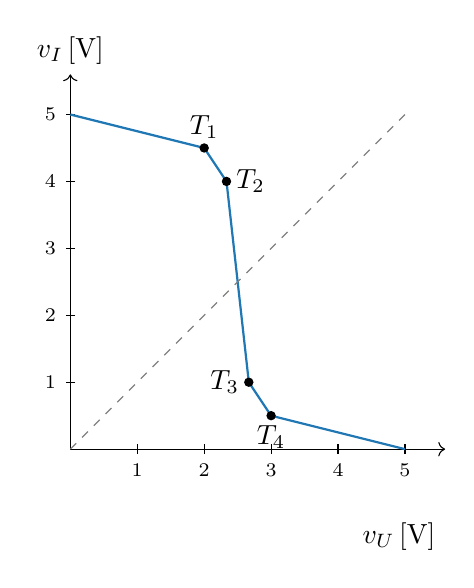
\begin{tikzpicture}[scale=.85]\draw[->] (0,0)--(5.6,0);\node[anchor=north east]at(5.6,-.95){$v_U\,[\mathrm V]$};\draw[->] (0,0)--(0,5.6) node[above]{$v_I\,[\mathrm V]$};\foreach \x in {1,...,5}{\draw (\x,.07)--(\x,-.07) node[below,font=\scriptsize]{\x};\draw (.07,\x)--(-.07,\x) node[left,font=\scriptsize]{\x};}\draw[Primary,thick] (0,5)--(2,4.5)--(2.3333333333333335,4)--(2.6666666666666665,1)--(3,0.5)--(5,0);\foreach\x/\y/\lab/\pos in{2/4.5/1/above,2.333333/4/2/right,2.666667/1/3/left,3/.5/4/below}{\fill(\x,\y)circle(2pt)node[\pos]{$T_\lab$};}\draw[dashed,gray](0,0)--(5,5);\end{tikzpicture}
\end{document}
